\documentclass[11pt]{article}

\usepackage{verbatim}
\usepackage{amsmath}
\usepackage{amssymb}
%\usepackage{psfrag}
\usepackage{setspace}
\usepackage[top=1in, bottom=1in, left=1.25in, right=1.25in]{geometry}
%\usepackage{fancyhdr}
\usepackage{subfigure}
\usepackage{graphicx}
\usepackage{cite}
\usepackage[squaren]{SIunits}
\usepackage{listings}
\usepackage{subfloat}
%\usepackage{hyperref}

%\pagestyle{fancy}
%\lhead{E155, Lab1}
%\chead{\today}
%\rhead{Sherman Lam}
%\renewcommand{\headrulewidth}{0.4pt}
%\lfoot{}
%\cfoot{}
%\rfoot{}


\setlength{\parindent}{0pt} 	% remove the silly paragraph indents

\begin{document}



% ---------------------------------------
% Name section
% ---------------------------------------
\begin{flushleft}
Sherman Lam
\\E155
\\ \today
\end{flushleft}


% ---------------------------------------
% Title
% ---------------------------------------
\begin{center}
\begin{Large}
\textbf{Lab 1 Report: Utility Board Assembly}
\end{Large}
\end{center}


% ---------------------------------------
% Start report
% ---------------------------------------


\section{Introduction}
\label{sec:intro}

This lab consisted of two main components: 
	\begin{enumerate} \itemsep0pt
		\item Assembling the development board
		\item Writing a simple program for interfacing LEDs and switches
	\end{enumerate}

In the first section of this lab, I assembled the E155 Utility Board from the provide kit. This board serves as a development board for a PIC32 microcontroller and a Cyclone III FPGA. The kit included basic through-hole components such as resistors, capacitors, switches, header pins, and LEDs. Other accessories included a VGA port, JTAG pins, and a jack for programming the PIC. The only surface-mount components were 3 voltage regulators (for 2.5V, 1.2V, and 3.3V). Upon completion of the assembly, I ran some basic checks to verify that the board performed as expected. \\

In the second section of this lab, I used Quartus II to design an interface between the DIP switches on the development board and several LEDs. The LEDs used were an LED bar on the development board and a 7-segment display that was wired off the board.


\section{Design and Testing Methodology}

\subsection{Hardware}

\subsubsection{Development Board}

The design of the development board was set by the course instructors and so it was simply assembled according to the provided lab instructions. As briefly mentioned in Section \ref{sec:intro}, several tests were run to verify that the hardware on the board functioned according to my expectations. The results included the following:

	\begin{description} \itemsep0pt
		\item[Pre-assembly Inspection ] No visible defects were found on the PCB or the components. Using a multimeter, no short was detected across Vin and GND.
		\item[Power Supply ] When the board was powered by a 5V regulated input, the outputs of the voltage regulators read within 0.05V of their nominal voltage outputs. 
		\item[Clock ] The output of the clock as measured by an oscilloscope was within 1MHz of the nominal frequency (40MHz).
		\item[LED Bar ] To check the LED bar's functionality, first the pin to one LED was connected (via a wire on the breadboard) to the pin of a switch. If the LED toggles with the switch, the LED was deemed functional. This test was repeated for all the LEDs. All LEDs performed as expected.
		\item[Switches ] To check the switches' functionality, first the pin to one LED on the LED bar was connected to the pin of one switch. If the LED toggles with the switch, the switch was deemed functional. This test was repeated for all the switches. All switches performed as expected.
		
		
	\end{description}


\subsubsection{7-Segment Display}


 Table \ref{tb:pin_mapping} shows the mapping between the segments of the 7-segment LED and output pins on the development board. These mappings were chosen to minimize wiring overlap on the breadboard. The layout of the segments on the display is shown in Figure \ref{figure:seven_segment_layout}.


\begin{table}[h]
\center
\begin{tabular}{|l|l|l|l|l|l|l|l|}
\hline
\multicolumn{8}{|c|}{7 - Segment Display Pin Mapping} \\ \hline
Pin       & P2  & P1  & P4  & P10  & P11  & P3  & P7  \\ \hline
Segment   & A   & B   & C   & D    & E    & F   & G   \\ \hline
\end{tabular}
\caption{Pin Mapping from development board to 7-segment display}
\label{tb:pin_mapping}
\end{table}


\begin{figure}[h!]
\centering
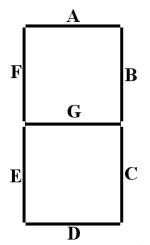
\includegraphics[scale=0.6]{seven_segment_layout.png}
\caption{Segment ordering of a 7-segment display. Image from E155 Lab1.}
\label{figure:seven_segment_layout}
\end{figure} 


In order to ensure that the logic on the output pins either settled on LOW or HIGH, a pull up resistor was placed on the output of each pin. $10k\Omega$ was selected because it can pull the logic level of a pin to HIGH without drawing much current. In addition, each segment was wired in series with its own current limiting resistor. The value of this resistor was chosen to be $220\Omega$ as determined by Equation \ref{eq:resistor}. This places the current draw per segment in the recommended $5mA$ to $20mA$ range. The schematic for a single segment of the display is shown in Figure \ref{figure:single_led}. The full schematic for the 7-segment display is shown in Figure \ref{figure:seven_segment}. The pinout for the 7-segment display is shown in Figure \ref{figure:seven_segment_pinout}. Since the display used has 2 7-segment displays, only half of the module was used (see Figure \ref{figure:seven_segment_image}). 


\begin{equation}
\label{eq:resistor}
R = V/I
  = (V_{supply}-V_{diode})/I
  = (3.3V - 0.7V)/10mA
  = 260\Omega
 \approx 220\Omega
\end{equation} 
		
\begin{figure}[h!]
\centering
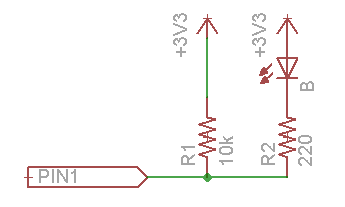
\includegraphics[scale=0.7]{single_led.png}
\caption{Schematic for segment B of the 7-segment display.}
\label{figure:single_led}
\end{figure} 

\begin{figure}[h!]
\centering
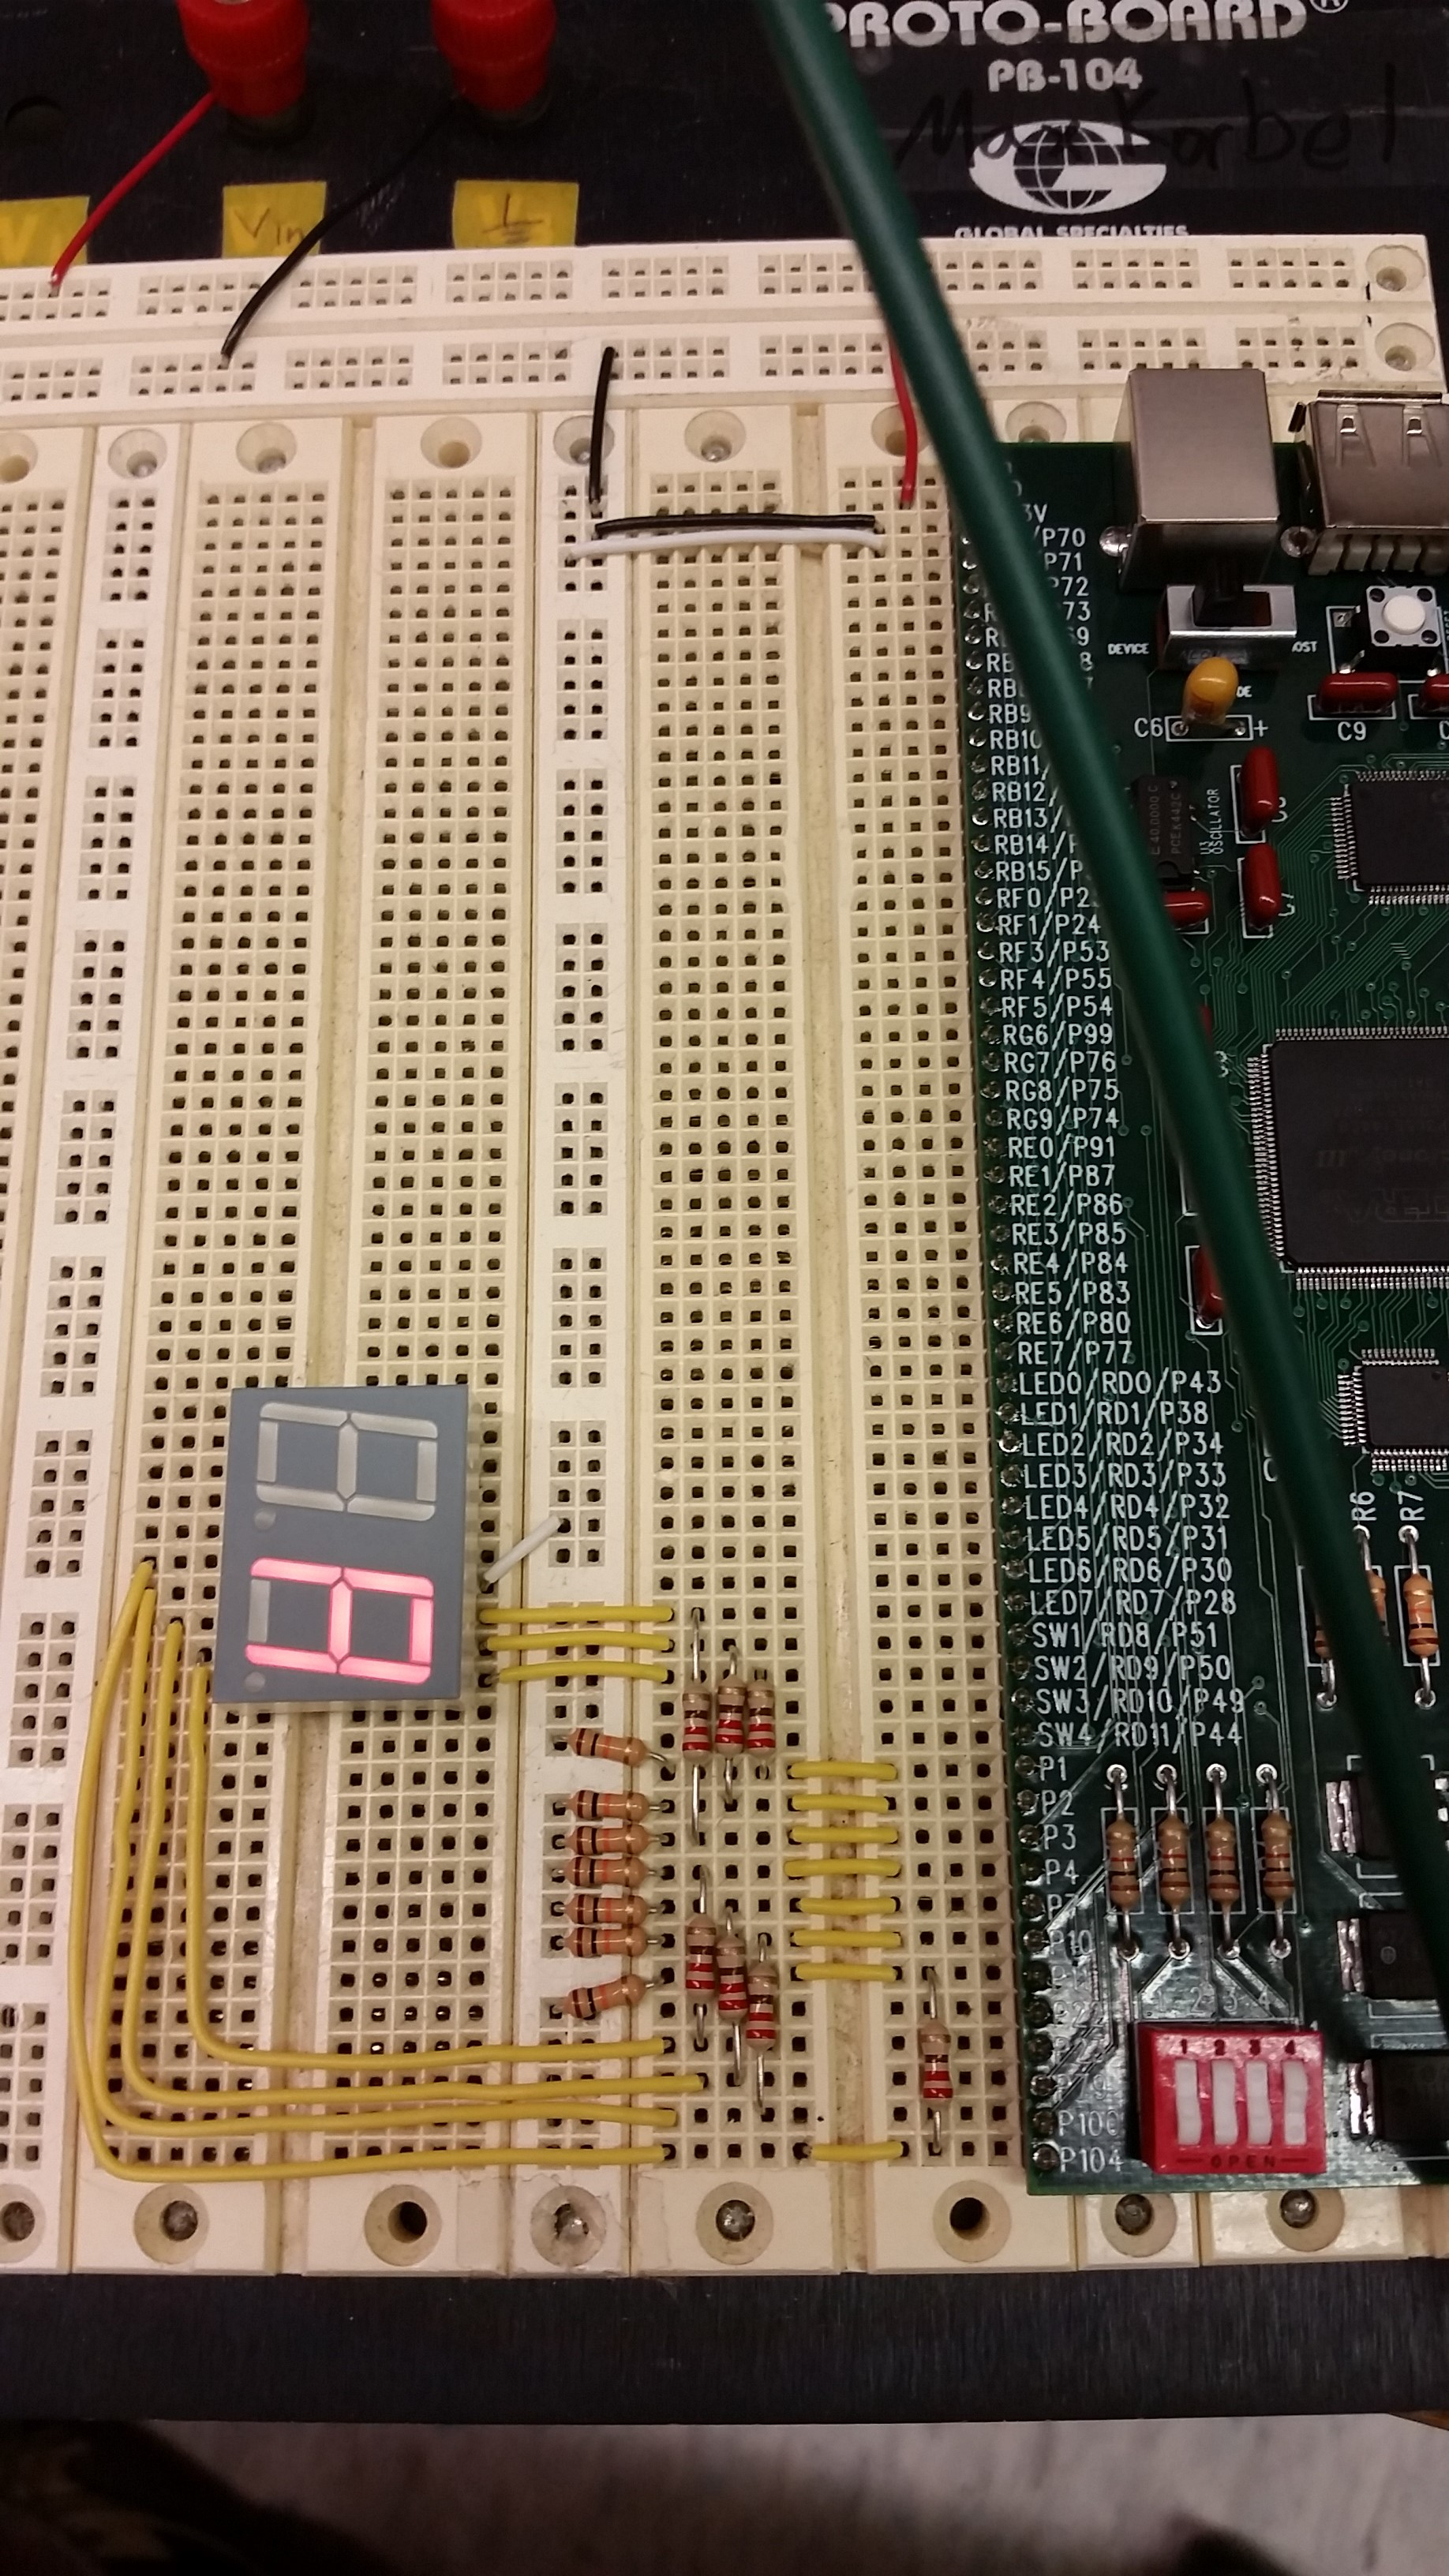
\includegraphics[scale=0.1]{seven_segment_image.jpg}
\caption{Image of the wired 7-segment display.}
\label{figure:seven_segment_image}
\end{figure} 

\clearpage

\subsection{Software}

\subsubsection{7-Segment Decoder}
\label{sec:software_7seg}

\begin{table}[h]
\centering
\begin{tabular}{|c|c|c|c|c|c|c|c|c|c|c|c|c|}
\hline
\multicolumn{13}{|c|}{7-Segment Display Truth Table}                                  \\ \hline
\multicolumn{5}{|c|}{Inputs}                      & \multicolumn{8}{c|}{Ouputs}       \\ \hline
s{[}3{]} & s{[}2{]} & s{[}1{]} & s{[}0{]} & (hex) & G & F & E & D & C & B & A & (hex) \\ \hline
0        & 0        & 0        & 0        & 0x0   & 1 & 0 & 0 & 0 & 0 & 0 & 0 & 0x40  \\ \hline
0        & 0        & 0        & 1        & 0x1   & 1 & 1 & 1 & 1 & 0 & 0 & 1 & 0x79  \\ \hline
0        & 0        & 1        & 0        & 0x2   & 0 & 1 & 0 & 0 & 1 & 0 & 0 & 0x24  \\ \hline
0        & 0        & 1        & 1        & 0x3   & 0 & 1 & 1 & 0 & 0 & 0 & 0 & 0x30  \\ \hline
0        & 1        & 0        & 0        & 0x4   & 0 & 0 & 1 & 1 & 0 & 0 & 1 & 0x19  \\ \hline
0        & 1        & 0        & 1        & 0x5   & 0 & 0 & 1 & 0 & 0 & 1 & 0 & 0x12  \\ \hline
0        & 1        & 1        & 0        & 0x6   & 0 & 0 & 0 & 0 & 0 & 1 & 0 & 0x02  \\ \hline
0        & 1        & 1        & 1        & 0x7   & 1 & 1 & 1 & 1 & 0 & 0 & 0 & 0x78  \\ \hline
1        & 0        & 0        & 0        & 0x8   & 0 & 0 & 0 & 0 & 0 & 0 & 0 & 0x00  \\ \hline
1        & 0        & 0        & 1        & 0x9   & 0 & 0 & 1 & 1 & 0 & 0 & 0 & 0x18  \\ \hline
1        & 0        & 1        & 0        & 0xA   & 0 & 0 & 0 & 1 & 0 & 0 & 0 & 0x08  \\ \hline
1        & 0        & 1        & 1        & 0xB   & 0 & 0 & 0 & 0 & 0 & 1 & 1 & 0x03  \\ \hline
1        & 1        & 0        & 0        & 0xC   & 0 & 1 & 0 & 0 & 1 & 1 & 1 & 0x27  \\ \hline
1        & 1        & 0        & 1        & 0xD   & 0 & 1 & 0 & 0 & 0 & 0 & 1 & 0x21  \\ \hline
1        & 1        & 1        & 0        & 0xE   & 0 & 0 & 0 & 0 & 1 & 1 & 0 & 0x06  \\ \hline
1        & 1        & 1        & 1        & 0xF   & 0 & 0 & 0 & 1 & 1 & 1 & 0 & 0x0E  \\ \hline
\end{tabular}
\caption{Truth table for 7-Segment LED decoder}
\label{table:7seg_decoder}
\end{table}

The software was written for simplicity. In particular, there are two approaches to the decoder of the 7-segment display. Both approaches start with a truth table with the state of the switches (s[3:0]) as the inputs and the state of the led segments (led[6:0]) as the outputs (see Table \ref{table:7seg_decoder}). Note that since this is a common anode 7-segment display, pulling a pin LOW will actually turn on the corresponding segment. The first approach is to write the state of each segment in terms of the inputs (either sum-of-products or product-of-sums form). The second approach uses a case structure to implement a lookup table. Every possible value for s[3:0] is mapped to a value for led[6:0]. \\

Quartus will theoretically optimize both approaches to similar (if not identical) logic blocks. Consequently, both will perform similarly in hardware. I chose to implement the lookup table since it is easier to code and less prone to coding mistakes. Also note that I configured the DIP switches with the LSB on the right hand side of the switch (switch 4). This yields an intuitive user interface. 


\subsubsection{LED bar decoder}
\label{sec:software_LEDbar}

The decoder for the LED bar is similar to that of the 7-segment display. Its functionality is described in Figure \ref{figure:led_bar_decoder}. \\

In order to flash the LED at 2.4Hz, I setup a counter that tracks the number of clock cycles that have elapsed. To "flash" an LED, the LED must first be toggled on and then off. This requires two clock cycles. So, to flash the LED at 2.4Hz, the LED needs to be toggled at 4.8Hz, or every $\frac{40MHz}{4.8Hz} = 83333333$ cycles. \\


\subsubsection{Testing and Flashing}

To check the logic output of my decoders, I simulated the module with ModelSim-Altera. The results are shown in Figure \ref{figure:wave}. The outputs agree with the behavior described in Sections \ref{sec:software_7seg} and \ref{sec:software_LEDbar}. The program was then flashed to PROM per lab instructions. This allows the FPGA to load the program whenever the board is turned on or reset. \\


\begin{figure}[h!]
\centering
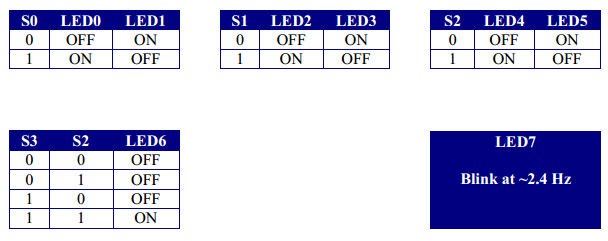
\includegraphics[scale=0.7]{led_bar.png}
\caption{Pin requirements for led bar decoder. Image from E155 Lab1.}
\label{figure:led_bar_decoder}
\end{figure} 


\begin{figure}[h!]
\centering
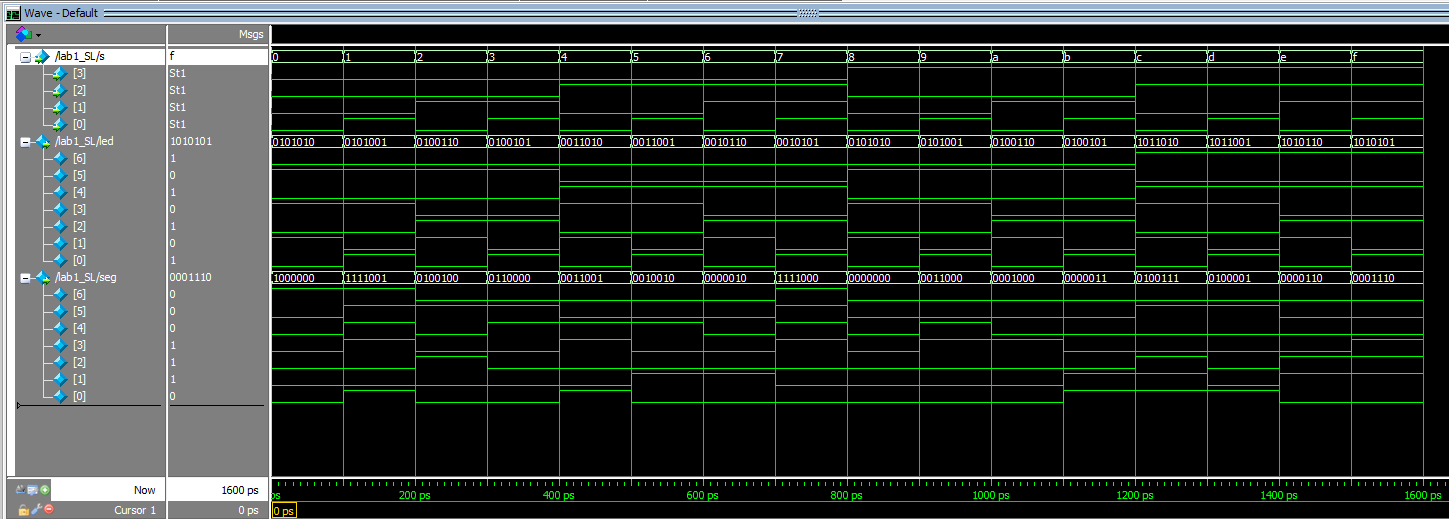
\includegraphics[scale=0.54, angle=90]{wave.png}
\caption{Simulation output of the module with ModelSim-Altera.}
\label{figure:wave}
\end{figure} 


\clearpage


\section{Technical Documentation}

This section provides the source code for this project and a full schematic for the 7-segment display wiring.

\subsection{System Verilog Code}

\small\begin{verbatim}

/* This module is the wrapper for the project. It instantiates
  an instance of the led bar decoder and 7 segment decoder
  
  Author: Sherman Lam
  Email: slam@g.hmc.edu
  Date: Sep 9, 2014
*/

module lab1_SL( input logic clk,        //clock
            input logic [3:0] s,        //4 DIP switches
            output logic [7:0] led,     //8 lights on LED bar
            output logic [6:0] seg);    //segments in 7-seg display
  
  //instance of the led bar decoder
  ledBarDecoder   bar(.clk(clk), .s(s), .led(led));   
  //instance of 7-seg display decoder
  led7Decoder     led7(.s(s), .seg(seg)); 

endmodule

/* This module decodes the switch inputs into an output for the 
  color bar on development board.
  s[3:0] = [sw3, ... ,sw1]
  led[7:0] = [led7, ... ,led0]
  
  Author: Sherman Lam
  Email: slam@g.hmc.edu
  Date: Sep 9, 2014
*/
module ledBarDecoder(input logic clk,
              input logic [3:0] s,
              output logic [7:0] led);
              logic [23:0] count = 24'b0;
              logic [23:0] period = 24'h7F2815;   //every 8333333 cycles of a 40MHz clock, the
                          	                      //7th led will toggle on or off. Yields a 
                          	                      //flashing rate of 2.4Hz
  
  always_ff @(posedge clk) begin
    if (count >= period) begin
      count <= 24'b0;
      led[7] = ~led[7];
    end
    else            
      count <= count + 1'b1;
  end
  
  always_comb begin
    led[1:0] = s[0] ? 2'b01 : 2'b10;
    led[3:2] = s[1] ? 2'b01 : 2'b10;
    led[5:4] = s[2] ? 2'b01 : 2'b10;
    led[6] = (s[3]&s[2]) ? 1'b1 : 1'b0;
  end

endmodule


/* This module decodes the switch inputs into an output for the 
  7 segment display on the development board.
  s[3:0] = [sw3, ... ,sw1]
  seg[6:0] = [g,f, ... ,b,a]
  
  Author: Sherman Lam
  Email: slam@g.hmc.edu
  Date: Sep 9, 2014
*/
module led7Decoder( input logic [3:0] s,  //4 DIP switches
              output logic [6:0] seg);    //segments in 7-seg display
              
  always_comb begin
    //lookup table for s-seg relationship
    case(s)
      4'h0:   seg = 7'b100_0000;      // 0x0
      4'h1:   seg = 7'b111_1001;      // 0x1
      4'h2:   seg = 7'b010_0100;      // 0x2
      4'h3:   seg = 7'b011_0000;      // 0x3
      4'h4:   seg = 7'b001_1001;      // 0x4
      4'h5:   seg = 7'b001_0010;      // 0x5
      4'h6:   seg = 7'b000_0010;      // 0x6
      4'h7:   seg = 7'b111_1000;      // 0x7
      4'h8:   seg = 7'b000_0000;      // 0x8
      4'h9:   seg = 7'b001_1000;      // 0x9
      4'ha:   seg = 7'b000_1000;      // 0xA
      4'hb:   seg = 7'b000_0011;      // 0xB
      4'hc:   seg = 7'b010_0111;      // 0xC
      4'hd:   seg = 7'b010_0001;      // 0xD
      4'he:   seg = 7'b000_0110;      // 0xE
      4'hf:   seg = 7'b000_1110;      // 0xF
      default: seg = 7'b111_1110;     // default to a dash
    endcase
   
  end
endmodule

\end{verbatim}


\begin{figure}[h!]
\centering
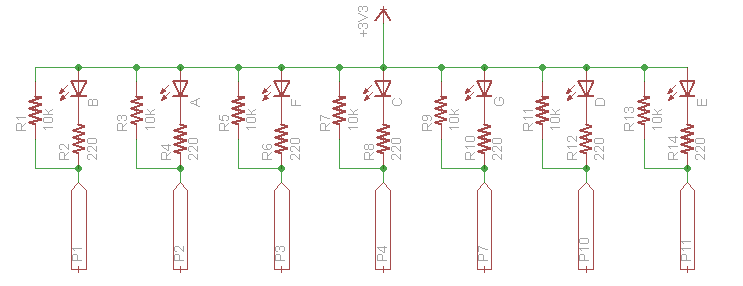
\includegraphics[scale=0.8]{seven_segment.png}
\caption{Schematic for full 7-segment display.}
\label{figure:seven_segment}
\end{figure} 


\begin{figure}[h!]
\centering
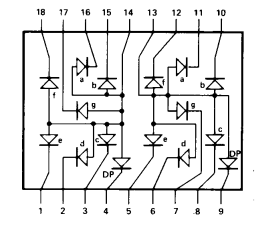
\includegraphics[scale=1]{seven_segment_pinout.png}
\caption{Pinout for a common anode 7-segment display. Source: Avago HDSP-F15x Series Datasheet, Digikey
}
\label{figure:seven_segment_pinout}
\end{figure} 



\clearpage

\section{Results and Discussion}

The program worked as expected. This indicates that the hardware (at least for the LEDs and switches) are all functioning. All aspects of the lab were completed. 



\section{Conclusion}

In this lab, I assembled the development board from the provide kit and programmed an interface between the onboard switches and several LEDs. The program was written in System Verilog, synthesized in Quartus II, and flashed on the FPGA through JTAG with Quartus' built in programmer. \\

Breakdown of time spent on lab:
\begin{description}
	\item[Assembling Board] 3.5hrs
	\item[Testing Hardware] 0.5hrs
	\item[Programming, Simulating, Debugging] 2hrs
	\item[Breadboarding] 1hrs
	\item[Relearning Latex] 2hrs
	\item[Writing Report] 4hrs
	\item[Total Time Spent] 13hrs
\end{description}


\end{document}
